\subsection{Sous section présentant les figures}

\subsubsection{Figure simple}

\blindtext[3]
\begin{figure}[htbp]
    \centering
    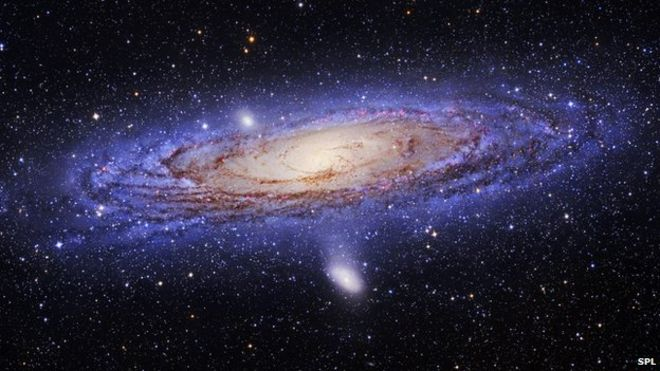
\includegraphics[width=0.8\textwidth]{image1.jpg}
    \caption{caption}%
    \label{fig:label}
\end{figure}

\subsubsection{Sous-figures}

\blindtext[4]
\begin{figure}[htbp]
    \centering
    \begin{subfigure}[t]{0.49\textwidth}
        \centering
        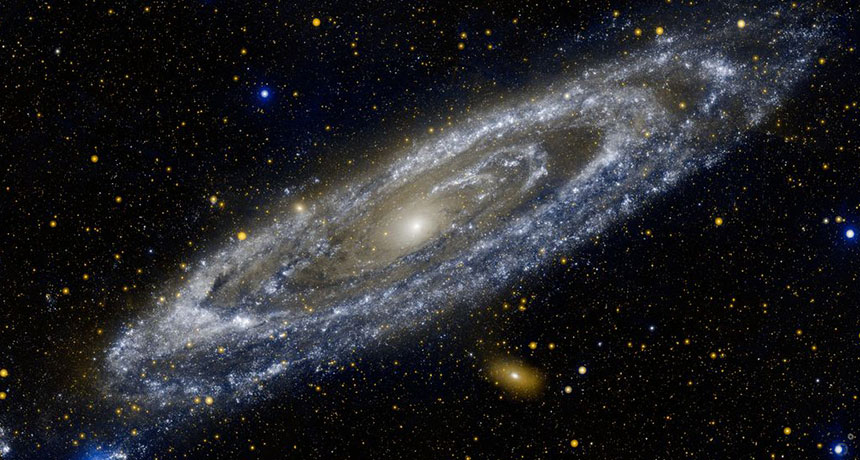
\includegraphics[width=0.9\textwidth]{image2.jpg}
        \caption{Very very long caption for a subfigure. This is setup with subcaption package.}%
        \label{fig:1a}
    \end{subfigure}
    \hfill
    \begin{subfigure}[t]{0.49\textwidth}
        \centering
        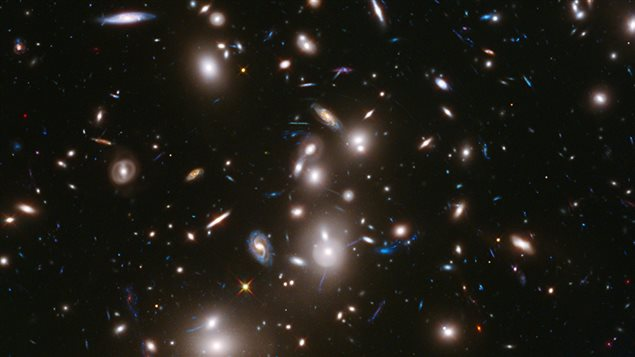
\includegraphics[width=0.9\textwidth]{image3.jpg}
        \caption{Short caption}%
        \label{fig:1b}
    \end{subfigure}
    \caption{Main figure caption. I add some text so that the caption is taking multiple lines.}%
    \label{fig:1}
\end{figure}

La \autoref{fig:1} possède deux sous figures~\ref{fig:1a} et~\ref{fig:1b}.

\subsubsection{Sous section avec du texte autour d'une figure}

\blindtext[1]

\begin{wrapfigure}{r}{0.5\textwidth} % l for left, r for right
    \centering
    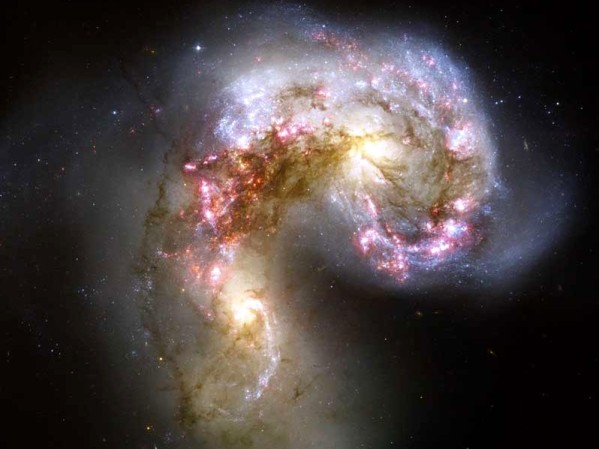
\includegraphics[width=0.4\textwidth]{image4.jpg}%
    \caption{caption}%
    \label{fig:wrapfig}
\end{wrapfigure}

\blindtext[2]

\subsubsection{Sous section avec un schéma Tikz}

\blindtext[5]
\begin{figure}[ht]
    \centering
    \includestandalone{coriolis}
    \caption{Force de Coriolis}%
    \label{fig:coriolis}
\end{figure}

\begin{figure}[ht]
    \centering
    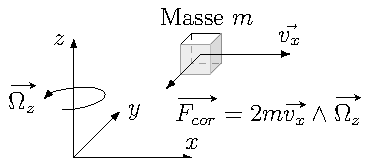
\includegraphics{coriolis}
    \caption{Force de Coriolis}%
    \label{fig:coriolisbis}
\end{figure}

